\frame{
\frametitle{2D Navier--Stokes equation: how much randomization noise?}

% \begin{figure}[htb!]
%     \centering
%     % \caption{{\bf 2D heat equation.} A (random) representative case of inverse and full forward solution obtained by $\TNetAE$ trained with 1 training sample coupled with data randomization of noise level $\sigma = 0.1$. $\TNetAE$ inverse solution is comparable to the Tikhonov (Tik) inverse counterpart, and both are consistent with the ground truth (True). $\TNetAE$ full forward solution is almost identical (in fact within 3 digits of accuracy) to the underlying true solution.}
%     \resizebox{.8\textwidth}{!}{
%     \begin{tabular*}{\textwidth}{c@{\hskip -0.01cm} c@{\hskip -0.01cm} c@{\hskip -0.01cm} c@{\hskip -0.01cm}}
%         \centering
%         \raisebox{-0.5\height}{$\ub_\text{Tikhonov}$} &
%         \raisebox{-0.5\height}{$\ub_{\TNetAE}$ } &
%         \raisebox{-0.5\height}{$\ub_\text{True}$}&
%         \raisebox{-0.5\height}{$\yb_{\TNetAE}$}
%         \\
%         \raisebox{-0.5\height}{\includegraphics[width = 0.25\textwidth]{Figs/Figs/2D_Poisson/Tik_test_sample_POI_sample.pdf}} &
%         \raisebox{-0.5\height}{\includegraphics[width = 0.25\textwidth]{Figs/Figs/2D_Poisson/Tnet_full_test_1sample_POI_sample.pdf}} &
%         \raisebox{-0.5\height}{\includegraphics[width = 0.25\textwidth]{Figs/Figs/2D_Poisson/True_test_sample_POI_sample.pdf}} &
%         \raisebox{-0.5\height}{\includegraphics[width = 0.25\textwidth]{Figs/Figs/2D_Poisson/Tnet_full_test_1sample_yobs_sample.pdf}}
%         \\
%         \raisebox{-0.5\height}{$\snor{\ub_\text{Tikhonov} - \ub_\text{True}}$} &
%         \raisebox{-0.5\height}{$\snor{\ub_{\TNetAE} - \ub_\text{True}}$ } &
%         \raisebox{-0.5\height}{$\yb_\text{True}$}&
%         \raisebox{-0.5\height}{$\snor{\yb_{\TNetAE} - \yb_\text{True}}$}
%         \\
%         \raisebox{-0.5\height}{\includegraphics[width = 0.25\textwidth]{Figs/Figs/2D_Poisson/Tik_test_error_sample_POI_sample.pdf}} &
%         \raisebox{-0.5\height}{\includegraphics[width = 0.25\textwidth]{Figs/Figs/2D_Poisson/Tnet_full_test_error_1sample_POI_sample.pdf}} &
%         \raisebox{-0.5\height}{\includegraphics[width = 0.25\textwidth]{Figs/Figs/2D_Poisson/True_test_1sample_yobs_sample.pdf}} &
%         \raisebox{-0.5\height}{\includegraphics[width = 0.25\textwidth]{Figs/Figs/2D_Poisson/Tnet_full_error_test_1sample_yobs_sample.pdf}}
%     \end{tabular*}
%     }
% \end{figure}
% \blueblox{Relative error of inverse solution over 500 test samples with different noise levels.}

\vspace{-9ex}
 
{
    \begin{figure}[htb!]
        \centering
        % \resizebox{.9\textwidth}{!}{
            \caption*{Relative error of inverse solution over 500 test samples with different noise levels.}
            % This file was created with tikzplotlib v0.10.1.
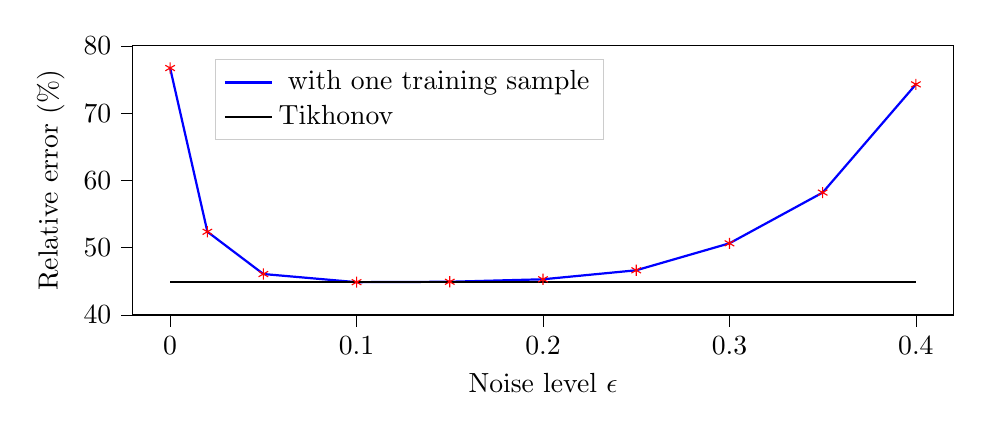
\begin{tikzpicture}[
        % Set the overall font size for the figure
        % font=\small,
        % Set the overall size of the figure
        % scale=1.2
    ]
    \definecolor{green01270}{RGB}{0,127,0}
    \definecolor{lightgray204}{RGB}{204,204,204}
    \definecolor{darkgray176}{RGB}{176,176,176}

    \begin{axis}[
            % Set the width and height of the axis
            width=12cm,
            height=5cm,
            % Other axis options...
            tick align=outside,
            tick pos=left,
            x grid style={darkgray176},
            xlabel={Noise level $\epsilon$},
            xmin=-0.02, xmax=0.42,
            xtick style={color=black},
            y grid style={darkgray176},
            ylabel={Relative error (\%)},
            ymin=0.4, ymax=0.8,
            ytick style={color=black},
            % Set font sizes for labels and ticks
            % xlabel style={font=\small},
            % ylabel style={font=\small},
            % tick label style={font=\small},
            % Set custom x ticks
            xtick={0,0.1,0.2,0.3,0.4},
            xticklabels={0,0.1,0.2,0.3,0.4},
            % Set custom y ticks
            ytick={0.4,0.5,0.6,0.7,0.8},
            yticklabels={40, 50, 60, 70, 80},
            % Optional: use scientific notation for y-axis
            % yticklabel style={/pgf/number format/fixed,/pgf/number format/precision=2},
            % Optional: rotate x-axis labels if they overlap
            % x tick label style={rotate=45,anchor=east},
            legend cell align={left},
            legend style={
                    fill opacity=0.8,
                    draw opacity=1,
                    text opacity=1,
                    at={(0.1,0.8)},
                    anchor=west,
                    draw=lightgray204
                },
        ]
        % ... rest of the plot code remains the same
        \addplot [thick, blue]
        table {%
                0 0.766974268854683
                0.02 0.523683383837577
                0.05 0.460874094482016
                0.1 0.448766294680066
                0.15 0.449361065883312
                0.2 0.453057512322396
                0.25 0.466427642188141
                0.3 0.506496804889437
                0.35 0.581920155123714
                0.4 0.7427047409309
            };
        \addlegendentry{$\TNetAE$ with one training sample}
        % \addlegendentry{1-sample training - $\text{ours}$}
        \addplot [thick, black]
        table {%
                0 0.449
                0.02 0.449
                0.05 0.449
                0.1 0.449
                0.15 0.449
                0.2 0.449
                0.25 0.449
                0.3 0.449
                0.35 0.449
                0.4 0.449
            };
        \addlegendentry{Tikhonov}
        \addplot [draw=red, fill=red, mark=asterisk, only marks]
        table{%
                x  y
                0 0.766974268854683
                0.02 0.523683383837577
                0.05 0.460874094482016
                0.1 0.448766294680066
                0.15 0.449361065883312
                0.2 0.453057512322396
                0.25 0.466427642188141
                0.3 0.506496804889437
                0.35 0.581920155123714
                0.4 0.7427047409309
            };
    \end{axis}
\end{tikzpicture}
        % }
        \figlab{Heat_noise_level}
    \end{figure}
}

}